% !TeX program = lualatex
\documentclass[10pt,xcolor=dvipsnames,aspectratio=169]{beamer}
\usepackage{fontspec}
\usepackage[fontset=fandol,scheme=plain]{ctex}
\usetheme[progressbar=frametitle,sectionpage=none,numbering=fraction]{metropolis}
% Preserve the supplied template's typography when Fira is installed.
% TeX Gyre Heros is the portable fallback used by this build.
\IfFontExistsTF{Fira Sans}{%
  \setsansfont{Fira Sans}[BoldFont={Fira Sans Medium}]
}{%
  \setsansfont{texgyreheros-regular.otf}[
    BoldFont=texgyreheros-bold.otf,ItalicFont=texgyreheros-italic.otf,
    BoldItalicFont=texgyreheros-bolditalic.otf]
}
\setmonofont{Latin Modern Mono}[Scale=MatchLowercase]
\usepackage{microtype,graphicx,booktabs,tabularx,amsmath,amssymb,amsfonts,amsthm,bm,mathtools}
\providecommand{\mathds}{\mathbb}
\usepackage{tikz,pgfplots}
\usetikzlibrary{arrows.meta,positioning,calc,fit,backgrounds}
% DESIGN COLORS
\definecolor{accent}{HTML}{7EBDC2} % accent color
\definecolor{bgcolor}{HTML}{FCFCFF} % background color
\definecolor{bgcolorAlt}{HTML}{ECF1FC} % alternative background color
\definecolor{fgcolor}{HTML}{222244} % foreground/text color

%
\setbeamercolor{normal text}{%
	fg=fgcolor,
	bg=bgcolor,
}
\setbeamercolor{alerted text}{%
	fg=accent,
}
\setbeamercolor{palette primary}{%
	use=normal text,
	fg=normal text.fg,
	bg=bgcolorAlt,%normal text.bg
}

\setbeamercolor{block title}{
	bg=bgcolorAlt,
}
\setbeamercolor{block body}{
	bg=bgcolorAlt,
}
\setbeamercolor{block title alerted}{%
	use={palette primary, alerted text},
	fg=palette primary.bg,
	bg=alerted text.fg
}
\setbeamercolor{block title example}{%
	use={block title, alerted text},
	bg=block title.bg,
	fg=alerted text.fg
}
%

% PLOT COLORS
%% Paul Tol High Contrast
\definecolor{plot0}{HTML}{004488}
\definecolor{plot1}{HTML}{DDAA33}
\definecolor{plot2}{HTML}{BB5566}
\definecolor{plot3}{HTML}{000000}
\definecolor{plot4}{HTML}{AAAAAA}

%% Paul Tol Vibrant
%\definecolor{plot0}{HTML}{EE7733}
%\definecolor{plot1}{HTML}{0077BB}
%\definecolor{plot2}{HTML}{33BBEE}
%\definecolor{plot3}{HTML}{EE3377}
%\definecolor{plot4}{HTML}{CC3311}
%\definecolor{plot5}{HTML}{009988}
%\definecolor{plot6}{HTML}{BBBBBB}
\makeatletter
\setbeamerfont{block body reference}{size=\scriptsize}
\setbeamerfont{block title reference}{size=\scriptsize}

\setbeamerfont{description item}{series=\mdseries}
\setbeamerfont{alerted text}{series=\bfseries\boldmath}

\setbeamerfont{bibliography item}{size=\small}
\setbeamerfont{bibliography entry author}{shape=\upshape,series=\mdseries,size=\small}
\setbeamerfont{bibliography entry title}{shape=\itshape,series=\mdseries,size=\small}
\setbeamerfont{bibliography entry journal}{shape=\upshape,series=\mdseries,size=\small}
\setbeamerfont{bibliography entry location}{shape=\upshape,series=\mdseries,size=\small}
\setbeamerfont{bibliography entry note}{shape=\upshape,series=\mdseries,size=\small}


\setbeamertemplate{title page}{
\begin{minipage}[b][\textheight]{\textwidth}
	\ifx\inserttitlegraphic\@empty\else\usebeamertemplate*{title graphic}\fi
	\vfill%
	\ifx\inserttitle\@empty\else\usebeamertemplate*{title}\fi
	\ifx\insertsubtitle\@empty\else\usebeamertemplate*{subtitle}\fi
	\usebeamertemplate*{title separator}

	\ifx\beamer@shortauthor\@empty\else\usebeamertemplate*{author}\fi
	\ifx\insertdate\@empty\else\usebeamertemplate*{date}\fi
	\ifx\insertinstitute\@empty\else\usebeamertemplate*{institute}\fi
	\vfil
	\vspace*{1mm}
\end{minipage}
}
\newcommand*{\seprule}{{\par\color{bgcolorAlt!90!fgcolor}\hrulefill\par\vspace*{1ex plus 0pt minus .5ex}}}
\makeatother
% Mathematical Writing
\DeclarePairedDelimiter{\abs}{\vert}{\vert}
\DeclarePairedDelimiter{\norm}{\Vert}{\Vert}
\DeclarePairedDelimiter{\ceil}{\lceil}{\rceil}
\DeclarePairedDelimiter{\floor}{\lfloor}{\rfloor}

\newcommand*{\inv}[1]{\ensuremath{#1^{-1}}}
\newcommand*{\positive}[1]{\ensuremath{\left[#1\right]^{+}}}

\newcommand*{\diff}{\ensuremath{\mathrm{d}}}
\newcommand*{\imag}{\ensuremath{\mathrm{j}}}
\newcommand*{\e}{\ensuremath{\mathrm{e}}}

\DeclareMathOperator*{\argmax}{arg\,max}
\DeclareMathOperator*{\argmin}{arg\,min}

%% change these to \mathbb, if you do not want to use the dsfont package
\newcommand*{\reals}{\ensuremath{\mathds{R}}} 
\newcommand*{\complexes}{\ensuremath{\mathds{C}}}
\newcommand*{\naturals}{\ensuremath{\mathds{N}}}
%%

\newcommand*{\expect}[2][]{\ensuremath{\mathbb{E}_{#1}\left[#2\right]}}

\newcommand*{\unif}{\ensuremath{\mathcal{U}}}
\newcommand*{\normaldist}{\ensuremath{\mathcal{N}}}


% THEOREMS
\theoremstyle{plain}% default
\newtheorem{thm}{Theorem}%[section]
\newtheorem{lem}{Lemma}
\newtheorem{prop}{Proposition}
\newtheorem{cor}{Corollary}

\pgfplotsset{compat=newest}

\pgfplotsset{legend style={fill=bgcolor,draw=fgcolor}}

\pgfplotscreateplotcyclelist{lineplot cycle}{ %
	{plot0, mark=*, thick, mark options=solid},
	{plot1, mark=triangle*, thick, mark options=solid},
	{plot2, mark=square*, thick, mark options=solid},
	{plot3, mark=diamond*, thick, mark options=solid},
	{plot4, mark=pentagon*, thick, mark options=solid},
}

\pgfplotsset{%
	betterplot/.style={
		width=.93\linewidth,
		height=.5\textheight,
		xlabel near ticks,
		ylabel near ticks,
		cycle list name=lineplot cycle,
		mark options=solid,
		xmajorgrids=true,
		xminorgrids=true,
		ymajorgrids=true,
%		major grid style={dotted},
		grid style={line width=.1pt, draw=gray!20},
		major grid style={line width=.25pt,draw=gray!30},
		legend cell align=left,
		legend style = {
			/tikz/every even column/.append style={column sep=0.33cm}
		},
	},
}
% Percentages only for displayed classification outcomes.
\newcommand{\LambdaRows}{%
fc8：固定 & 54.21\% & 54.21\% & 0.50 \\
fc8：第 1 轮起自适应 & 54.97\% & 51.32\% & 3.64 \\
fc8：第 41 轮起自适应 & 54.21\% & 53.58\% & 0.87 \\
conv5+fc8：固定 & 56.48\% & 52.58\% & 0.50 \\
conv5+fc8：第 50 轮起自适应 & 55.97\% & 53.58\% & 6.94 \\
}

\newcommand{\ResnetRows}{%
No CORAL & 100 & 80.00\% & 80.00\% & +0.00 pp \\
logits & 37 & 81.01\% & 78.49\% & +2.52 pp \\
pooled & 100 & 80.38\% & 80.00\% & +0.38 pp \\
pooled+logits & 42 & 80.25\% & 78.11\% & +2.14 pp \\
layer4 & 100 & 79.87\% & 80.00\% & -0.13 pp \\
layer4+logits & 42 & 81.76\% & 78.11\% & +3.65 pp \\
}

\newcommand{\SubRows}{%
无适应 & $0$ & 46.54\% \\
global & $0.5\G$ & 53.84\% \\
global\_quarter & $0.25\G$ & 54.09\% \\
local & $0.5\LC$ & 42.14\% \\
mixed & $0.25\G+0.25\LC$ & 49.56\% \\
}

\newcommand{\GeometryRows}{%
Global CORAL & 53.84\% & 0.12058 & 0.326 & 0.427 \\
Local CORAL & 42.14\% & 0.01053 & 0.331 & 0.229 \\
LMMD & 66.16\% & 0.03481 & 0.102 & 0.591 \\
}


\setbeamersize{text margin left=8mm,text margin right=8mm}
\setbeamerfont{frametitle}{size=\large,series=\bfseries}
\setbeamerfont{title}{size=\LARGE,series=\bfseries}
\setbeamerfont{subtitle}{size=\normalsize}
\setbeamerfont{block title}{size=\normalsize,series=\bfseries}
\setbeamerfont{block body}{size=\small}
\setbeamerfont{footnote}{size=\tiny}
\setbeamercolor{alerted text}{fg=plot0}
\setbeamercolor{progress bar}{fg=accent,bg=bgcolorAlt}
\setbeamertemplate{navigation symbols}{}
\hypersetup{colorlinks=true,urlcolor=plot0,linkcolor=plot0,pdftitle={从全局统计到类别几何：Deep CORAL 与子域对齐实验汇报},pdfauthor={张以禾}}
\graphicspath{{figures/}}
\newcommand{\src}[1]{\par\vfill{\fontsize{5.5}{6.4}\selectfont\color{fgcolor!65}来源：#1\par}\vspace{-1mm}}
\newcommand{\takeaway}[1]{\par\vspace{1mm}{\color{plot0}\bfseries #1}\par}
\newcommand{\fullfig}[1]{\centering\includegraphics[width=\linewidth,height=.69\textheight,keepaspectratio]{#1}}
\newcommand{\smallfig}[2][.56]{\centering\includegraphics[width=\linewidth,height=#1\textheight,keepaspectratio]{#2}}
\newcommand{\G}{\mathcal L_{\mathrm{G}}}
\newcommand{\LC}{\mathcal L_{\mathrm{C}}}
\newcommand{\M}{\mathcal L_{\mathrm{LMMD}}}
\newcommand{\CE}{\mathcal L_{\mathrm{CE}}}
\newcommand{\sg}{\operatorname{sg}}
\newcommand{\ESS}{\operatorname{ESS}}
\newcolumntype{Y}{>{\raggedright\arraybackslash}X}
\newcolumntype{P}[1]{>{\raggedright\arraybackslash}p{#1}}
\tikzset{box/.style={draw=plot0!25,fill=bgcolorAlt,rounded corners=1.5mm,align=center,inner sep=2mm,font=\small},
  flow/.style={-{Stealth[length=2mm]},thick,draw=plot0},
  tag/.style={font=\scriptsize,align=center,text=fgcolor}}
\title{从全局统计到类别几何}
\subtitle{Deep CORAL、子域对齐与 LMMD / DSAN 的实验探索}
\author{张以禾}
\institute{Office-31 · Amazon $\rightarrow$ Webcam}
\date{2026 年 10 月 16 日}

\begin{document}
\maketitle
\section{CORAL 实验}

\begin{frame}{Deep CORAL 原实验复现}
\centering
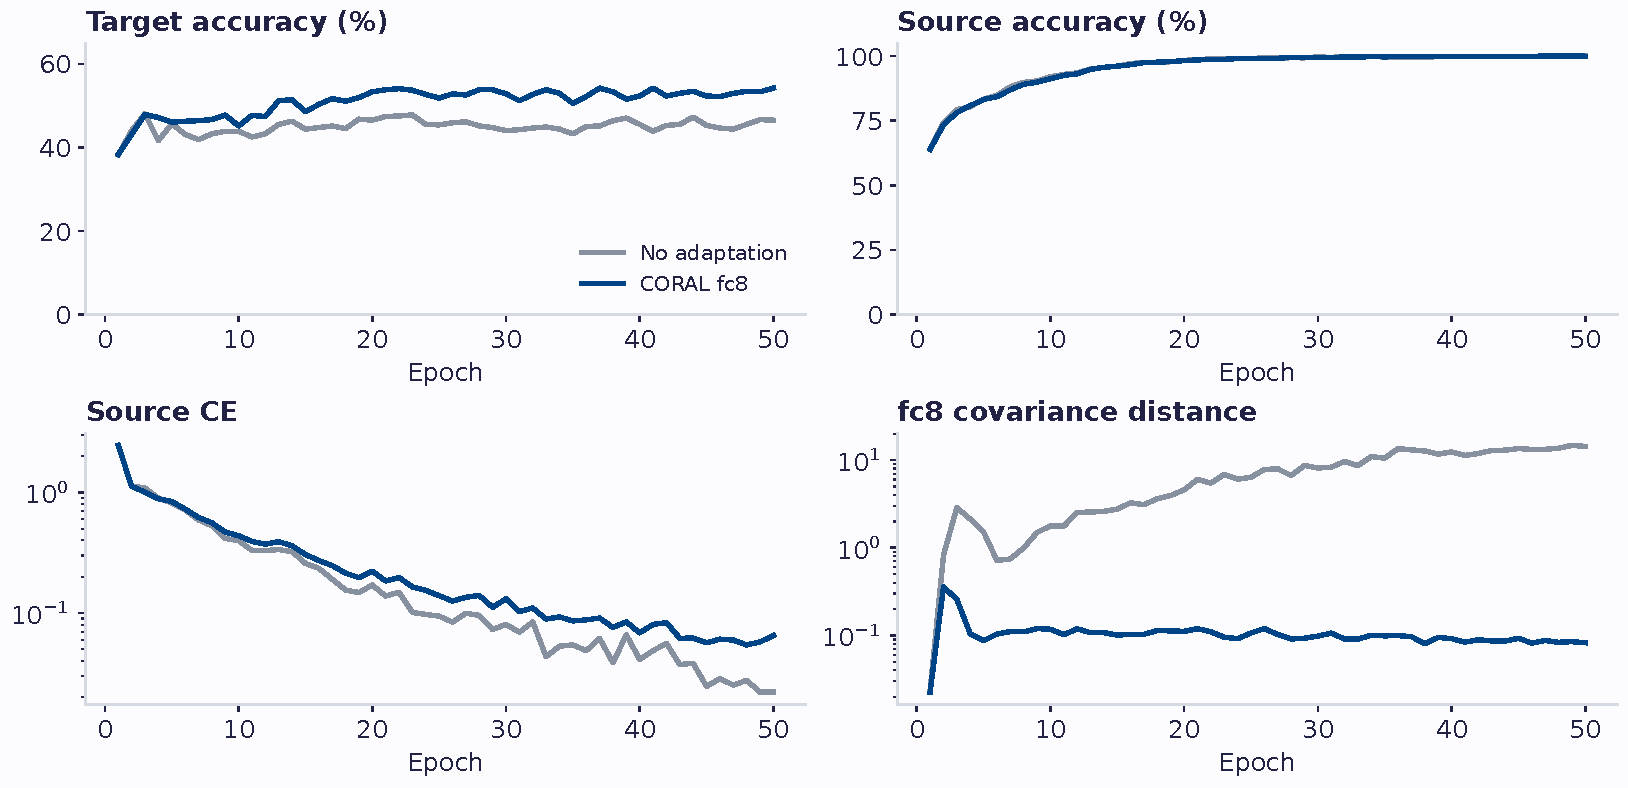
\includegraphics[width=\linewidth,height=.82\textheight,keepaspectratio]{baseline.pdf}
\end{frame}

\begin{frame}[t]{多层 CORAL 联合对齐}
\small
\[
\mathcal L=\CE+\frac{\lambda}{|\mathcal A|}\sum_{\ell\in\mathcal A}
\frac{\norm{C_s^{(\ell)}-C_t^{(\ell)}}_F^2}{4D_\ell^2},\qquad\lambda=0.5.
\]
\begin{tabularx}{\linewidth}{@{}lYY@{}}
\toprule
层 & 对齐对象 & 实际损失系数 \\
\midrule
conv5 & 空间位置上的 256 维通道特征 & 单层：0.5 \\
fc6 / fc7 & 4,096 维 Linear 输出，ReLU 前 & 双层：各 0.25 \\
fc8 & 31 维分类 logits & 三层：各 $1/6$ \\
\bottomrule
\end{tabularx}
\vspace{3mm}
\begin{itemize}
  \item 单层：conv5、fc6、fc7、fc8。
  \item 联合：conv5+fc8、fc6+fc7、fc6+fc8、fc7+fc8、fc6+fc7+fc8。
  \item AlexNet V1，Amazon$\to$Webcam，seed=42，batch=128，固定 50 轮。
\end{itemize}
\src{reports/data/layer\_results.csv；多层损失取均值。}
\end{frame}

\begin{frame}[t]{多层 CORAL：conv5+fc8 的正确率最高}
\fullfig{alex_layers.pdf}
\takeaway{conv5+fc8：55.09\%；fc8：54.21\%；无适应：46.54\%。更多对齐层没有带来单调改善。}
\src{AlexNet 位置实验，第 50 轮目标正确率。}
\end{frame}

\begin{frame}[t]{自适应 $\lambda$：梯度范数平衡}
\small
在共享 conv5 参数上计算梯度范数，EMA decay=0.9；$\lambda=e^s$：
\[
g_{\rm CE}=\norm{\nabla\CE}_2,\quad g_{\rm G}=\norm{\nabla\G}_2,\quad
\boxed{J_\lambda=(\lambda\overline g_{\rm G}-\overline g_{\rm CE})^2}.
\]
独立 Adam（lr=0.01）学习 $s$；模型更新时将 $\lambda$ detach。
\vspace{2mm}
\begin{tabularx}{\linewidth}{@{}Yrrr@{}}
\toprule
配置 & 最佳正确率 & 最终正确率 & 最终 $\lambda$ \\
\midrule
\LambdaRows
\bottomrule
\end{tabularx}
\takeaway{全程自适应 fc8 的最终正确率下降；联合组的峰值也没有提高。}
\src{reports/data/lambda\_results.csv；fc8 为 50 轮，conv5+fc8 为 100 轮。}
\end{frame}

\begin{frame}[t]{启用自适应后：$\lambda$ 激增，CORAL loss 快速下降}
\smallfig[.51]{lambda_failure.pdf}
\small
\begin{itemize}
  \item 第 50 轮启用后：$\lambda$ 从 0.5 升至 \textbf{6.94}；原始 $\G$ 从 0.0853 降至 \textbf{0.0167}。
  \item 出现 $\G\to0$ 的趋势，与论文强调避免的退化方向一致；对齐值下降未改善最佳正确率。
\end{itemize}
\takeaway{该自适应方案无效，依然采用固定 $\lambda=0.5$。}
\src{conv5+fc8 逐轮日志；\href{https://arxiv.org/pdf/1607.01719}{Deep CORAL \S3.2} 强调分类与对齐约束的平衡。}
\end{frame}

\begin{frame}[t]{停止条件：分类损失与加权 CORAL 损失平衡}
\small
记每轮训练均值 $a_e=\CE$、$b_e=0.5\G$，分别维护 decay=0.5 的 EMA。
\[
\delta(a,b)=\frac{|a-b|}{\max(a,b,10^{-12})}.
\]
\begin{block}{规则与条件}
从第 20 轮起，\textbf{当轮与 EMA 的相对差距均 $\le25\%$}，\textbf{连续两轮}满足则停止；最大预算 100 轮。
\end{block}
\vspace{1mm}
\textbf{设计目的：}保持固定适应强度，以训练内信号判断两项约束是否达到平衡，减少过长训练。
\par\vspace{3mm}
\textbf{conv5+fc8 结果：}日志回放在第 \textbf{58} 轮触发，正确率 \textbf{56.48\%}；第 100 轮为 52.58\%。原始 / EMA 差距分别为 13.17\% / 15.72\%。
\src{reports/data/early\_stop\_results.csv；停止信号只读取训练损失。}
\end{frame}

\begin{frame}[t]{ResNet-50：CORAL 的额外收益不明显}
\small
ImageNet V2，batch=32，共享 BN；$\lambda=0.5$，双层各 0.25；使用相同停止规则。
\vspace{2mm}
\begin{tabularx}{\linewidth}{@{}Yrrrr@{}}
\toprule
配置 & 停止轮 & 正确率 & 同轮对照正确率 & 同轮增益 \\
\midrule
\ResnetRows
\bottomrule
\end{tabularx}
\vspace{2mm}
无 CORAL 已达到 \textbf{80.00\%}；单独 pooled / layer4 对齐基本没有改善，含 logits 的配置有小幅收益。
\takeaway{在这种更先进的预训练网络上，CORAL 并未带来明显的性能跃迁。}
\src{reports/resnet50/summary.csv；同轮对照采用一致的共享 BN 配置。}
\end{frame}

\section{CORAL 子域对齐}

\begin{frame}[t]{子域对齐：分别匹配同一类别的两域分布}
\small
第 $c$ 类子域为源域与目标域中属于该类别的样本；目标类别由模型概率估计。
\[
\text{全局对齐：}\mathcal D(P_s,P_t)
\qquad\longrightarrow\qquad
\text{子域对齐：}\frac1C\sum_{c=1}^{C}\mathcal D(P_s^c,P_t^c).
\]
\begin{columns}[T,onlytextwidth]
\column{.48\textwidth}
\begin{block}{全局统计混合了什么？}
整体协方差同时包含类内变化和类间中心结构。\par
不同类别的域偏移可能相互掩盖。
\end{block}
\column{.48\textwidth}
\begin{block}{子域对齐匹配什么？}
源域类别 $c$ 对应目标域类别 $c$，分别建立统计量并对齐。\par
目标域使用软类别权重，而非真实标签。
\end{block}
\end{columns}
\[
\mathcal L=\CE+\lambda\,\mathbb E_c[\mathcal D(P_s^c,P_t^c)].
\]
\src{\href{https://arxiv.org/pdf/2106.09388}{DSAN，第 III 节}：按类别划分相关子域。}
\end{frame}

\begin{frame}[t]{参考 DSAN 实现 CORAL 子域对齐}
\small
借用 DSAN 的类别软权重，将其统计目标替换为\textbf{逐类协方差差异}：
\[
p_{jc}=\sg[\operatorname{softmax}(z_j^t)_c],\quad
a^s_{ic}=\frac{\mathbf1[y_i^s=c]}{\sum_r\mathbf1[y_r^s=c]},\quad
a^t_{jc}=\frac{p_{jc}}{\sum_rp_{rc}}.
\]
\[
\mu_d^c=\sum_i a^d_{ic}z_i^d,\qquad
C_d^c=\frac{\sum_i a^d_{ic}(z_i^d-\mu_d^c)(z_i^d-\mu_d^c)^\top}{1-\sum_i(a^d_{ic})^2}.
\]
\[
\boxed{\LC=\frac1{|\mathcal V|}\sum_{c\in\mathcal V}\frac{\norm{C_s^c-C_t^c}_F^2}{4D^2}}.
\]
\begin{itemize}
  \item AlexNet fc8 的 31 维 logits；目标权重 detach，特征路径反传。
  \item 有效类要求：源支持 $\ge2$、目标 top-1 支持 $\ge2$、目标 ESS $\ge2$。
\end{itemize}
\src{src/core/subdomain\_coral.py；类别权重参考 DSAN，协方差目标为本实验自定义。}
\end{frame}

\begin{frame}[t]{CORAL 子域对齐：未产生正向效果}
\small
统一初始化、batch=128；适应组前十轮均使用 $0.5\G$，第 11 轮切换。
\vspace{2mm}
\begin{tabularx}{\linewidth}{@{}Ycr@{}}
\toprule
配置 & 第 11--50 轮适应项 & 第 50 轮正确率 \\
\midrule
\SubRows
\bottomrule
\end{tabularx}
\vspace{3mm}
\begin{itemize}
  \item local 相对 global \textbf{下降 11.70 pp}。
  \item mixed 在保留全局系数 0.25 的情况下，仍比 global\_quarter \textbf{低 4.53 pp}。
\end{itemize}
\takeaway{更细的类别划分没有改善分类，直接沿用类内协方差目标反而损害正确率。}
\src{reports/subdomain\_coral/lmmd/summary.csv；均为固定第 50 轮结果。}
\end{frame}

\section{LMMD 实验}

\begin{frame}[t]{实验 DSAN 的 LMMD：AlexNet 与 ResNet-50}
\small
LMMD 沿用类别软权重，匹配同类样本的\textbf{核均值嵌入}：$\mathcal L=\CE+\lambda\M$。
\vspace{2mm}
\begin{tabularx}{\linewidth}{@{}P{26mm}YY@{}}
\toprule
 & AlexNet & ResNet-50 V2 \\
\midrule
对齐表示 & fc8：31 维 logits & 2048 $\to$ 256 bottleneck $\to$ 31；对齐 256 维 \\
训练配置 & batch=128，6 步 / 轮 & batch=32，源域驱动 87 步 / 轮 \\
适应项 & 前 10 轮 $0.5\G$；后 40 轮 $0.5\M$ & 无 CORAL 预热；$\lambda(e)$ 渐增至 0.5 \\
学习率 & 0.001 / 0.01，固定 & 0.001 / 0.01 / 0.01，作者衰减 \\
结果选择 & 固定第 50 轮 & 每轮目标评估选最佳；30 轮无提升停止 \\
\bottomrule
\end{tabularx}
\vspace{3mm}
两组均使用作者的\textbf{五核 RBF}与共享类别规则；ResNet 按作者代码使用裁剪 / 翻转且不加 Normalize。
\src{reports/subdomain\_coral/lmmd/protocol.md；reports/resnet50\_lmmd/protocol.md。}
\end{frame}

\begin{frame}[t]{AlexNet + LMMD：正确率提高到 66.16\%}
\fullfig{alex_lmmd_accuracy.pdf}
\takeaway{固定第 50 轮：全局 CORAL 53.84\%，子域 CORAL 42.14\%，LMMD 66.16\%。}
\src{同一 AlexNet / fc8 / 十轮预热配置；LMMD 相对全局 CORAL +12.33 pp。}
\end{frame}

\begin{frame}[t]{ResNet-50 + LMMD：最佳正确率 93.71\%}
\fullfig{resnet_lmmd_accuracy.pdf}
\takeaway{第 42 轮最佳 93.71\%；第 72 轮停止为 93.58\%。}
\src{ResNet-50 V2 + 256 维 bottleneck；最佳轮按目标正确率选择；论文 DSAN A$\to$W 为 $93.6\pm0.2\%$。}
\end{frame}

\section{LMMD 的理论优势与反思}

\begin{frame}[t]{LMMD 的设计：类别条件下的核均值匹配}
\small
令 $k(x,y)=\langle\phi(x),\phi(y)\rangle_{\mathcal H}$，同类两域的核均值差为
\[
\boxed{\M=\frac1{|\mathcal U|}\sum_{c\in\mathcal U}
\left\|\sum_i a^s_{ic}\phi(z_i^s)-\sum_j a^t_{jc}\phi(z_j^t)\right\|_{\mathcal H}^2}.
\]
将平方范数展开，得到实际计算形式：
\[
\begin{aligned}
M_c={}&\sum_{i,i'}a^s_{ic}a^s_{i'c}k(z_i^s,z_{i'}^s)
+\sum_{j,j'}a^t_{jc}a^t_{j'c}k(z_j^t,z_{j'}^t)\\
&-2\sum_{i,j}a^s_{ic}a^t_{jc}k(z_i^s,z_j^t),\qquad
\M=\frac1{|\mathcal U|}\sum_cM_c.
\end{aligned}
\]
\begin{itemize}
  \item 前两项描述域内相似度，交叉项拉近跨域的同类核分布。
  \item $\mathcal U$ 为源真实类别与目标 top-1 类别的交集；域内求和包含对角线。
\end{itemize}
\src{\href{https://arxiv.org/pdf/2106.09388}{DSAN，Eq. (5)--(8)}；作者 LMMD 实现。}
\end{frame}

\begin{frame}[t]{区别一：协方差遗漏类别中心，LMMD 能感知位置差异}
\small
固定类别权重时，逐域平移不改变类内协方差：
\[
C_a(Z+\mathbf1v^\top)=C_a(Z).
\]
因此，两域同类可以具有\textbf{相同协方差、不同中心}，而 $\LC=0$。
\vspace{2mm}
\begin{block}{核均值会检测这种差异}
线性核下：$M_c=\norm{\mu_s^c-\mu_t^c}_2^2$。\par\vspace{2mm}
单核 RBF 下，以集中在 $u\ne v$ 的同类分布为例：
\[
M_c=k(u,u)+k(v,v)-2k(u,v)
=2\bigl(1-e^{-\norm{u-v}^2/\beta}\bigr)>0.
\]
\end{block}
\takeaway{子域 CORAL 对“类别放在哪里”没有直接约束；LMMD 保留了这类位置信息。}
\src{基于两种实际目标函数的推导；$\beta>0$，同类分布的示例用于说明中心差异。}
\end{frame}

\begin{frame}[t]{区别二：RBF 核比较的结构比二阶协方差更充分}
\small
类条件 CORAL 只匹配\textbf{中心化二阶矩}，相同均值 / 协方差仍可对应不同分布。
\[
e^{-\norm{x-y}^2/\beta}
=e^{-\norm x^2/\beta}e^{-\norm y^2/\beta}
\sum_{r=0}^{\infty}\frac{(2/\beta)^r}{r!}(x^\top y)^r.
\]
RBF 核使用无限维非线性特征，能够区分均值、协方差以外的分布结构。
\begin{block}{总体层面的可识别性}
固定带宽的高斯核是特征核（characteristic kernel）：
\[
\operatorname{MMD}_k^2(P,Q)=0\quad\Longleftrightarrow\quad P=Q.
\]
\end{block}
\takeaway{同样按类别分组，LMMD 匹配的是更完整的分布信息，而非仅类内波动。}
\src{\href{https://www.jmlr.org/papers/v13/gretton12a.html}{Gretton et al., A Kernel Two-Sample Test (2012), \S2}；DSAN。}
\end{frame}

\begin{frame}[t]{区别三：自适应带宽弱化“只缩小幅度”的捷径}
\small
拼接两域批次为 $u_1,\ldots,u_n$，作者使用五个核之和：
\[
b_0=\frac{\sum_{r\ne q}\norm{u_r-u_q}^2}{n(n-1)},\quad b=\max(\sg[b_0],10^{-12}),\quad
k(x,y)=\sum_{h=0}^{4}e^{-\norm{x-y}^2/(b2^{h-2})}.
\]
固定类别权重，共同缩放 $Z\mapsto sZ$，且每批同步重估带宽：
\[
\LC(sZ_s,sZ_t)=s^4\LC(Z_s,Z_t),\qquad
\frac{\norm{sx-sy}^2}{s^2b}=\frac{\norm{x-y}^2}{b}.
\]
\begin{itemize}
  \item CORAL 的绝对距离可以仅因特征收缩而迅速减小。
  \item 带宽下限未触发时，LMMD 的核值对共同正缩放保持不变；五核同时覆盖多个距离尺度。
  \item 这是重估带宽后的前向性质；实现中带宽 detach，目标 softmax 仍每批更新。
\end{itemize}
\takeaway{LMMD 不会仅因为两域特征一起变小，就在前向数值上得到更好的对齐值。}
\src{作者 LMMD 带宽 $b/4,b/2,b,2b,4b$；缩放推导以固定权重与正缩放为条件。}
\end{frame}

\begin{frame}[t]{区别四：LMMD 更适合类别支持稀疏的小批次}
\small
\begin{tabularx}{\linewidth}{@{}P{28mm}YY@{}}
\toprule
 & 自实现子域 CORAL & LMMD 作者规则 \\
\midrule
需要估计的统计量 & 每类协方差及有限样本修正 & 每类加权核均值 \\
源域 / 目标支持 & 各至少 2 个支持样本 & 共享类各至少 1 个即可 \\
权重集中度限制 & 目标 ESS $\ge2$ & 无 ESS 门槛 \\
批内类别利用 & 先过滤协方差不可靠的类别 & 可利用单样本共享类 \\
\bottomrule
\end{tabularx}
\vspace{3mm}
\begin{itemize}
  \item 类别较多、batch 较小时，LMMD 不必依赖稳定的逐类协方差估计。
  \item 相同 $\lambda$ 不代表相同梯度强度；本轮两种目标的支持规则、带宽与优化尺度同时不同。
\end{itemize}
\takeaway{LMMD 的优势同时来自统计目标和可用类别范围。}
\src{src/core/subdomain\_coral.py；src/core/lmmd.py。}
\end{frame}

\begin{frame}[t]{反思：子域划分不够，还要选对统计目标}
\small
\begin{tabularx}{\linewidth}{@{}Yrrrr@{}}
\toprule
方法 & 正确率 & 类内协方差距离 & 类中心方向距离 & 软权重纯度 \\
\midrule
\GeometryRows
\bottomrule
\end{tabularx}
\vspace{2mm}
\begin{itemize}
  \item 子域 CORAL 的协方差距离最小，正确率却最低；\textbf{更小的二阶差异不是更好的分类}。
  \item LMMD 的中心方向更接近、软分组更准确，与其更充分的分布约束相符。
  \item LMMD 仍要与 CE 联合：全体特征完全相同也会使其为零；类别判别性由分类约束共同维持。
\end{itemize}
\takeaway{本轮有效的是“类别软分组 + 核分布匹配 + 源域判别”，而非单独把全局 CORAL 拆成逐类 CORAL。}
\src{固定第 50 轮事后诊断；方向距离越低越接近，纯度越高越好；目标真值仅用于这些诊断。}
\end{frame}

\end{document}
